\chapter{CAMB, Initial Setup}

To reiterate, our first research goal is to investigate the impact of massive
neutrinos on the power spectrum more closely. This will help us to understand
how to incorporate $\omega_\nu$ into the evolution mapping framework.
In this chapter, we will familiarize ourselves with our chosen Boltzmann 
solver, CAMB, and introduce various important settings. Although CAMB was
written in Fortran-90, we will be exclusively accessing CAMB through its
Python wrappers, as CL is a Python package. 

%%%
\begin{comment}
\textcolor{blue}{
I hope to, in painstaking detail, cover many of the lines of the code that I
have written to interface with CAMB. I will include plots to indicate, at
every step, what incorrect settings cause the power spectrum to look like (or,
for subtler errors, what the error curves looked like compared to Ariel's
results, which I treated as a sort of ``ground truth''). This should also be a
good example to flex my physics interpretation skills: why does this incorrect
setting produce this undesired pattern?}

\textcolor{blue}{You might think that this is sort of an inappropriate 
section
for a master's thesis (especially since I have in mind that this be a lengthy 
section), but I would like to include it unless you feel very strongly. After
all, I spent several months of the project debugging at least ten different 
ways that slight and major errors in the various settings led to 
irreconcilable results.}
\end{comment}
%%%

\textcolor{orange}{Ariel recommends
just talking about the correct lines, don't talk about what happens when
they're wrong.}

%%% C'mon, Ariel's GOT to let me have this plot. It's a big open question!
\begin{comment}
In figure \ref{fig: spectrum_type}, we can see that requesting of the wrong
power spectrum type can in some low-$\omega_\nu$ cases yields errors so low
that we might accidentally overlook them. This error pattern is easily
recognizable and is a consequence of the definition of the power spectrum: the
Fourier transform  of the two-point correlation function. ...Okay, I'm still 
thinking about this. I don't understand %yet, but I'll be sure to ask you if I
%I'm still struggling about it.
\end{comment}
%%%

%s Now discuss individual settings

To set up a power spectrum calculation, CAMB requires a
\verb|CAMBparams| object which stores all the settings from accuracy levels
to cosmological parameter values. In the following sections, \verb|pars| 
refers to the \verb|CAMBparams| object within our code.

\section{Universal Settings}

First, we will motivate settings that are universal across runs. These are 
mostly contained in the helper function \\
\verb|apply_universal_output_settings| in the
CL script \verb|camb_interface.py|.

Although CAMB also offers CMB spectra, we are interested in the
matter power spectrum. Therefore, \verb|apply_universal_output_settings|  
first disables CMB calculations:

\verb|pars.WantCls = False| \quad CMB transfer function

\verb|pars.Want_CMB = False| \quad temperature and polarization spectra

\verb|pars.Accuracy.AccuratePolarization = False|

\verb|pars.DoLensing = False| \quad calculates lensing of the CMB

\verb|pars.WantScalars = False| \quad calculates E modes of CMB polarization, 
which are generated by density perturbations \cbib{Basu}.

\

Next, we need to specify that we want the \textit{linear} matter power 
spectrum:

\verb|pars.NonLinear = camb.model.NonLinear_none|

% Why is CAMB set up this way anyway? Why do I have to put in a model object 
% instead of simply flipping a Boolean? {probably not a relevant question for
% this thesis.}

\

The helium mass fraction $Y_\text{He}$ is not a focus of this work and is left
at the standard value:

\verb|pars.YHe = 0.24| \quad \cbib{Cooke}

\

%s k range

\verb|pars.Transfer.kmax = 10.0| \quad in absolute units,
the smallest scale at which we evaluate the power spectrum.
\footnote{Technically, this is the smallest scale at which we evaluate the
\textit{transfer} function, but for our purposes the distinction is
unimportant. For an introduction to the transfer function, see \citet{FECS}.} 

We note that our limit is extremely small. The smallest scale probed by
currently available cosmological data is $k \approx 3$ Mpc$^{-1}$
\cbib{Aghanim}. We use this limit with potential future surveys in mind.

\

Last, we set the accuracy with which CAMB should calculate power spectra.
Although higher accuracies should require greater computation time, we only
need to generate one training set in order to produce an emulator. Therefore,
computation time invested now will result in an emulator which is more
accurate and equally fast.

\verb|pars.Accuracy.lAccuracyBoost = 3| \quad requests more multipoles in the 
Boltzmann hierarchy. \textcolor{orange}{Whatever that is}

\verb|pars.Accuracy.AccuracyBoost = 3| 

The second line is explained in the CAMB documentation only as a ``general 
accuracy setting effecting [\textit{sic}] everything related to step sizes 
etc.'' \citet{Lesgourges} compares CLASS and CAMB at various values for this
attribute and find that at 3, the code precision already reaches the 0.1\% 
level. \textcolor{orange}{But what, more specifically, does it do? And it may
be a good idea to test the emulator with a much better precision: the value of
12 is the largest meaningful value in the Lesgourges paper.}

\

One additional universal setting is handled in the function
\verb|input_cosmology|, which translates a cosmology dictionary into 
the \verb|CAMBparams| object \verb|pars|. The cosmology dictionary is
intended to store cosmological parameters in a more user-friendly format.
All cosmology dictionaries should follow the same structure in order to be 
correctly interpreted by the various functions in CL. The required keys are 
described in table~\ref{tab: cosmology_dictionary}; all
values should be floating point numbers. The user is advised to print out
cosmology dictionaries with the \verb|print_cosmology| function in the
\verb|user_interface.py| script, which will automatically ignore unused keys
and resolve extreme roundoff cases.

% Address unused (OmL) and sometimes used (OmK) parameters
% Remind the user that, to "leave values at default for cassL," he can
% simply copy model0 and modify that. Use the function default_cosmology()

\begin{table}[ht!]
\centering
\begin{tabular}{l|l}
\hline
Key & Significance \\ \hline
'ombh2' & $\omega_b$ \\
'omch2' & $\omega_c$ \\
'n\_s' & $n_s$ \\
'A\_s' & $A_s$ \\
'OmK' & $\Omega_K$ \\
'h' & $h$ \\
'w0' & $w_0$ in the CPL EoS for DE \\
'wa' & $w_a$ in the CPL EoS for DE \\
'sigma12' & $\sigma_{12}$\footnotemark \\
'omnuh2' & $\omega_\nu$ \\
'mnu' & $\sum_i m_{\nu, i}$ \\
'nnu\_massive' & Number of massive $\nu$ species \\ \hline
\end{tabular}
 \cprotect\caption[Cosmology Dictionary Keys]{Keys
 	expected by the functions in
 	the \verb|camb_interface.py| script. Keep in mind that any additional
 	keys that may appear when printing out a cosmology dictionary
 	(such as 'OmL') are generally not used and therefore may be inconsistent.
 	with other parameter values.}
 \label{tab: cosmology_dictionary}
\end{table}
 	
\footnotetext{Specifying a $\sigma_{12}$ value will not affect the power
spectrum returned by \verb|evaluate_cosmology|. Instead, this field is used
by the \verb|direct_eval_cell| and \verb|interpolate_cell| functions
(section~\ref{sec: generate_emu_data}).}

The \verb|input_cosmology| function implements the following additional
settings universal to all of our power spectra:

\verb|tau=0.0952| \quad specified in the call to \verb|pars.set_cosmology|.
$\tau$ describes the optical depth to the CMB. \textcolor{orange}{What kinds 
of parameters are $Y_\text{He}$ and $\tau$ in evolution mapping?
Do they affect the power spectrum at all?}


\section{Dark Energy Settings}

The \verb|input_dark_energy| function modifies the input \verb|pars| object
according to the input DE EoS parameters, $w_a$ and $w_0$. For the standard
Planck best-fit cosmology, $w_0 = -1$ and $w_a = 0$. For this special case,
referred to as cosmological constant $\Lambda$, we use the two-
fluid approximation. Wherever the EoS departs from this, we use instead the
more flexible parametrized post-Friedmann (PPF) model.

\textcolor{orange}{What is the difference between the ``fluid'' and ``PPF''
models?? Can you show that these two models agree when $w_a$ and $W-0$ are
given by best fit values?}

\section{Neutrino Settings}

%s Setting omega_nu

As mentioned in section~\ref{sec: param_glossary}, we are interested in the
parameter $\omega_\nu$ and will need to vary it. CAMB does not seem to accept
$\omega_\nu$ values directly, in what may be a bug. For example, setting
\verb|pars.omnuh2| does not affect the return values of

\textcolor{orange}{This is wrong. Andrea was able to use camb.set\_params to 
get the desired omnuh2!!}

\verb|camb.get_results(pars).get_matter_power_spectrum|.

However, it may simply be the case that the \verb|omnuh2| attribute is
intended only as an output field. The \verb|pars.set_cosmology| function
accepts \verb|mnu| (the sum of the masses of the different neutrino flavors,
$\sum_i m_{\nu, i}$ \textcolor{orange}{in eV? Or what are the units??}),
which then updates the value of \verb|pars.omnuh2|.
In order to transform between the two, we have included in
\verb|camb_interface.py| the two convenience functions
\verb|omnuh2_to_mnu| and \verb|mnu_to_omnuh2|, which merely present the 
internal logic of CAMB in an isolated and user-accessible way.

\textcolor{orange}{Explain the equation being used here:}

\begin{equation}
\sum_i m_{\nu, i}
=
\omega_\nu \, x_\nu \, \left( \frac{3}{N_\nu^\text{eff}} \right)^{3/4}
,\end{equation}

where $x_\nu$ is \textcolor{orange}{the mysterious ``neutrino mass fac''} and
$N_\nu$ is the effective number of massive neutrino species. The standard
particle model predicts this to be 3.046 \cbib{Archidiacono}.

%s Neutrino peculiarities
The standard particle model specifies three flavors of neutrino which are
coherent superpositions of three mass eigenstates. It is not well understood
whether the mass associated with the $\nu_3$ eigenstate is greater or less
than that of the $\nu_1$ and $\nu_3$ eigenstates. The ``normal'' neutrino
\textit{mass hierarchy} places the greatest mass in the $\nu_3$
eigenstate; the ``inverted'' mass hierarchy places the smallest mass there. 
CAMB supports both of these hierarchies as well as a third: ``degenerate''
assigns the same mass to every eigenstate.\cbib{Qian}.

For this demonstration project, we will use the simple setup of a single
massive neutrino eigenstate. Consequently, the choice of hierarchy is 
important
only in scaling the mass value we assign this flavor. For example, if we use
the normal hierarchy with the same value of $\sum_i m_{\nu, i}$, then the
power spectrum will look as though we had used the degenerate hierarchy with
a smaller value of $\sum_i m_{\nu, i}$. In other words, it appears that the
most massive neutrino flavor dominates the impact of massive neutrinos on the
power spectrum.

Recall from section~\ref{sec: neutrino_problem} that we will need to keep
track of a MEMNeC for every massive-neutrino cosmology for which we wish to
compute a power spectrum. To make this easier, we have included the function
\verb|balance_neutrinos_with_CDM| which takes as parameters a cosmology
dictionary and a value for $\omega_\nu$, \verb|new_omnuh2|. If
\verb|new_omnuh2| is zero, the function returns the cosmology's MEMNeC.
If \verb|new_omnuh2| is nonzero and the cosmology has $\omega_\nu = 0$, 
the function returns the MEMNeC's massive-neutrino counterpart.

Lastly, we use the function \verb|specify_neutrino_mass| to add entries to
a cosmology dictionary before requesting power spectra.
It takes a cosmology dictionary, an $\omega_\nu$ value, and the number of
massive neutrinos--not the effective number $N_\nu^\text{eff}$, but a simple 
integer. It records these, as well as the corresponding
$\sum_i m_{\nu, i}$ value, in a copy of the cosmology
dictionary. \verb|specify_neutrino_mass| is not a helper function 
automatically called by others, but needs to be called whenever computing
power spectra with CL.

\textcolor{orange}{How can I justify using $N_\nu^\text{eff} = 3.046$ for the
``mnu'' conversion while I use $N_\nu^\text{massive} = 1$ for the call to
``set\_cosmology''? The truth is that it doesn't really matter, right? since
CAMB uses these as the default values anyway. But why do they do that?}

This function is important because the cosmologies that we use to test our
code in section~\ref{sec: CAMB_validation} are the Aletheia models,
which do not specify a neutrino configuration. Furthermore, since we use 
Aletheia model 0 as a set of default values for emulator training later on,
this function will remain important.

\section{Convenience Functions}

% camb\_interface.py

The helper functions of the previous chapters, as well as some additional
manipulations of \verb|pars|, are bundled together in several larger
functions which are designed to be used in the emulator pipeline. These
functions return power spectra given an input cosmology dictionary and
therefore represent a great starting point for beginners experimenting with
the CL code.

CL offers two main approaches to evaluating a power spectrum given an input
cosmology dictionary. The \textit{direct evaluation} approach uses CAMB's 
\verb|get_matter_power_spectrum| function, which evaluates a cosmology over
an array of explicit $z$ values. This approach is used by the top-level
function \verb|evaluate_cosmology|, which takes as inputs a 
cosmology dictionary, an array of redshifts, the desired resolution of the
power spectrum, and whether to use Hubble
units.\footnote{The user is encouraged to disregard the
\verb|fancy_neutrinos| flag for this function, as it relates
to an investigation into CAMB's handling of various neutrino properties.}
Remember that the use of Hubble units affects both the $x$- and
$y$-axes (compare again figures~\ref{fig: h_units}
and~\ref{fig: without_h_units}.). The resolution is specified according to
\verb|k_points|, the number of points at which to evaluate
the power spectrum. CAMB applies this value by sampling the scale range at
\verb|k_points| logarithmically spaced points.

The \verb|get_CAMB_pspectrum| 
function is a helper for this approach and is not likely to be otherwise 
needed by a typical user. For users interested in
developing their own interfaces with CAMB, we mention two further
settings in the call to \verb|get_matter_power_spectrum| which are not
modifiable through CL functions:

\verb|minkh=1e-4 / pars.h| and \verb|maxkh=10.0 / pars.h|
\quad sets the desired
range of inverse scales to $10^{-4} \leq k$ Mpc $\leq 10$. These values were
selected to fully encompass the various probes of the power spectrum without
extending the range too far into unexplored regions \cbib{Aghanim}. 

\verb|var1=`delta_nonu'| and \verb|var2=`delta_nonu'| requests the power
spectrum of cold matter with itself.

The second main approach is to use a 2D spline interpolation object returned
by CAMB's \verb|get_matter_power_interpolator|. The user gives a
range of $z$ and $k$ values over which to interpolate and then may request
the power spectrum at any $(z, k)$ location within this space from the
interpolator. This approach is handled by the CL function
\verb|cosmology_to_PK_interpolator|, which accepts a cosmology dictionary,
a set of redshifts, a maximum $k$ value, and whether to use Hubble units.
The function accepts redshifts stored in an array in order to maximize
compatibility with \verb|evaluate_cosmology|, although the meaning is slightly
different here: since the number of $z$ values in the array determines the
resolution of the interpolator, the user desiring maximum accuracy is
encouraged to input 150 redshift values, which is the maximum allowed by CAMB.

The \verb|get_CAMB_interpolator| function is a helper for this approach and is 
not 
likely to be otherwise needed by a typical user. For users interested in
developing their own interfaces with CAMB, we mention two further
settings in the call to \\
\verb|get_matter_power_interpolator| which are not
modifiable through CL functions:

\verb|nonlinear=False| (\textcolor{orange}{Why are we specifying the linear
power spectrum in two cases?)} \quad requests linear power spectrum.

\verb|var1=`delta_nonu'| and \verb|var2=`delta_nonu'| requests the power
spectrum of cold matter with itself.


\section{Verifying Our Settings}
\label{sec: CAMB_validation}

In order to confirm that our power spectra are viable for emulator training,
we need to ensure they are at least accurate at the level of error on CAMB
itself. We test the various \verb|camb_interface.py| functions described in
this chapter against two other CAMB implementations: one from Andrea Pezzotta,
using a different interpolator setup, and the other from Ariel G. S\'{a}nchez,
accessing the native Fortran without any wrapper. The CL function
\verb|load_benchmark| function exists only to store S\'{a}nchez's results in
memory.

We compare the power spectra produced by our CAMB calls for the four
approximate $\omega_\nu$ values\footnote{These values are
accessible through the CL global array \verb|OMNUH2_FLOATS|.}
$6.356 \cdot 10^{-4}$, $2.149 \cdot 10^{-3}$,
$6.356 \cdot 10^{-3}$, and $1 \cdot 10^{-2}$. For each
$\omega_\nu$, we test each of the first seven Aletheia cosmologies for 
a total of 28 models.

To call CAMB on Aletheia models in a convenient and structured way, we have
introduced two additional \verb|camb_interface.py| functions:
\verb|parse_redshifts| function returns the array of redshift values $z_i$
associated with each Aletheia model, where $i$ is the column of the file
\verb|cosmologies.dat| (included with CL). These $z_i$ are defined such that

\begin{equation}
\sigma_{12}(\text{model a}, z_{i, \text{model a}})
=
\sigma_{12}(\text{model b}, z_{i, \text{model b}})
,\end{equation}

Since the Aletheia models share values for the shape parameters, the
evolution mapping relation gives:

\begin{equation}
P_L(k, \text{model a}, z_{i, \, \text{model a}})
=
P_L(k, \text{model b}, z_{i, \, \text{model b}})
,\end{equation}

Therefore, a first sanity check for any code accessing CAMB is to reproduce
figure~\ref{fig: ev_mapping_demo} using the $z_i$ to control for $\sigma_{12}$
across the different Aletheia models. The function \verb|parse_redshifts|
returns the $z_i$ for a particular model in descending order--i.e. oldest
to newest. This is not only the order within \verb|cosmologies.dat|--CAMB
will automatically sort input redshift arrays to this order, so to avoid
confusion we keep redshift arrays in this order from the start.

CL's \verb|boltzmann_battery| function creates a battery of CAMB power
spectra according to the same
format\footnote{Refer to the docstring for a detailed breakdown of this
format.} in which S\'{a}nchez's results are
returned by \verb|load_benchmark|. Since the evaluation of 28 models can take
some time, the user is encouraged to skip any uninteresting indices--
\verb|skips_omega| for $\omega_\nu$ values, \verb|skips_model| for
Aletheia models, and \verb|skips_snapshots| for snapshots. The snapshot index
is equivalent to a backwards-running redshift index, so the last snapshot
corresponds to a redshift of zero. The \verb|skips_model| array should always
include 8, as that model cannot be processed in the latest (as of October 2,
2023) version of CL.

Since S\'{a}nchez's power spectra were evaluated at 1000 points, we call
\\
\verb|boltzmann_battery| with \verb|k_points=1000|. The errors are miniscule 
and recorded in figure XXY. 

\begin{figure}[ht!]
  \centering
  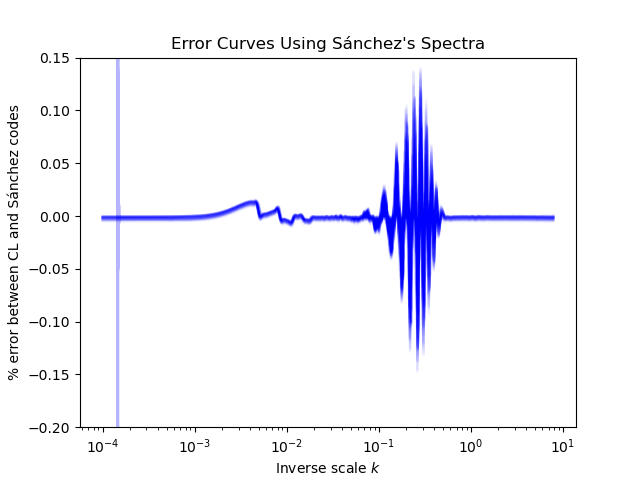
\includegraphics[width=\textwidth]{err_on_CL/Ariel}
  \caption[CL Consistency]{35 error curves, spanning
  	7 Aletheia models and 5 $\omega_\nu$ values.}
  \label{fig: Ariel_errs}
\end{figure}

The code described in this chapter lays the foundation for the rest of the
work. All of the power spectra that we use will be computed via CL.

% Aletheia Model 8 has not been integrated into our code suite yet. We can’t 
% handle its DE weirdness. Instead of bringing up and then discarding model 8, 
% we shouldn’t mention it at all.

% The plot should consist of an error swarm, one against Ariel, one against
% Andrea.

